\documentclass{article}
\usepackage[margin=1in]{geometry}
\usepackage{hyperref}
\usepackage{amsmath,amsfonts,amssymb,amsthm,commath,dsfont}
\usepackage{enumitem}
\usepackage{framed}
\usepackage{xspace}
\usepackage{microtype}
\usepackage{float}
\usepackage[round]{natbib}
\bibliographystyle{plainnat}
\usepackage{cleveref}
\usepackage[dvipsnames]{xcolor}
\usepackage{graphicx}
\usepackage{listings}
\usepackage[breakable]{tcolorbox}
\tcbset{breakable}
\usepackage{mathtools}
\usepackage{caption}
\usepackage{subcaption}
\def\b1{\boldsymbol{1}}

\newcommand{\colbar}{\rule[-3mm]{.3mm}{1.5em}}
\newcommand{\rowbar}{\rule[.5ex]{1.5em}{.3mm}}
\DeclareMathOperator{\rank}{rank}
\def\balpha{\boldsymbol{\alpha}}
% following loops stolen from djhsu
\def\ddefloop#1{\ifx\ddefloop#1\else\ddef{#1}\expandafter\ddefloop\fi}
% \bbA, \bbB, ...
\def\ddef#1{\expandafter\def\csname bb#1\endcsname{\ensuremath{\mathbb{#1}}}}
\ddefloop ABCDEFGHIJKLMNOPQRSTUVWXYZ\ddefloop

% \cA, \cB, ...
\def\ddef#1{\expandafter\def\csname c#1\endcsname{\ensuremath{\mathcal{#1}}}}
\ddefloop ABCDEFGHIJKLMNOPQRSTUVWXYZ\ddefloop

% \vA, \vB, ..., \va, \vb, ...
\def\ddef#1{\expandafter\def\csname v#1\endcsname{\ensuremath{\boldsymbol{#1}}}}
\ddefloop ABCDEFGHIJKLMNOPQRSTUVWXYZabcdefghijklmnopqrstuvwxyz\ddefloop

% \valpha, \vbeta, ...,  \vGamma, \vDelta, ...,
\def\ddef#1{\expandafter\def\csname v#1\endcsname{\ensuremath{\boldsymbol{\csname #1\endcsname}}}}
\ddefloop {alpha}{beta}{gamma}{delta}{epsilon}{varepsilon}{zeta}{eta}{theta}{vartheta}{iota}{kappa}{lambda}{mu}{nu}{xi}{pi}{varpi}{rho}{varrho}{sigma}{varsigma}{tau}{upsilon}{phi}{varphi}{chi}{psi}{omega}{Gamma}{Delta}{Theta}{Lambda}{Xi}{Pi}{Sigma}{varSigma}{Upsilon}{Phi}{Psi}{Omega}{ell}\ddefloop

\newcommand\T{{\scriptscriptstyle\mathsf{T}}}
\def\diag{\textup{diag}}

\DeclareMathOperator*{\argmin}{arg\,min}
\DeclareMathOperator*{\argmax}{arg\,max}

\def\SPAN{\textup{span}}
\def\tu{\textup{u}}
\def\R{\mathbb{R}}
\def\E{\mathbb{E}}
\def\Z{\mathbb{Z}}
\def\be{\mathbf{e}}
\def\nf{\nabla f}
\def\veps{\varepsilon}
\def\cl{\textup{cl}}
\def\inte{\textup{int}}
\def\dom{\textup{dom}}
\def\Rad{\textup{Rad}}
\def\lsq{\ell_{\textup{sq}}}
\def\hcR{\widehat{\cR}}
\def\hcRl{\hcR_\ell}
\def\cRl{\cR_\ell}
\def\hcE{\widehat{\cE}}
\def\cEl{\cE_\ell}
\def\hcEl{\hcE_\ell}
\def\eps{\epsilon}
\def\1{\mathds{1}}
\newcommand{\red}[1]{{\color{red} #1}}
\newcommand{\blue}[1]{{\color{blue} #1}}
\def\srelu{\sigma_{\textup{r}}}
\def\vsrelu{\vec{\sigma_{\textup{r}}}}
\def\vol{\textup{vol}}
\def\sr{\sigma_r}

\newcommand{\ip}[2]{\left\langle #1, #2 \right \rangle}
\newcommand{\mjt}[1]{{\color{blue}\emph{\textbf{[MJT:}~#1~\textbf{]}}}}

\newtheorem{fact}{Fact}
\newtheorem{lemma}{Lemma}
\newtheorem{claim}{Claim}
\newtheorem{proposition}{Proposition}
\newtheorem{theorem}{Theorem}
\newtheorem{corollary}{Corollary}
\newtheorem{condition}{Condition}
\theoremstyle{definition}
\newtheorem{definition}{Definition}
\theoremstyle{remark}
\newtheorem{remark}{Remark}
\newtheorem{example}{Example}

\def\hw{\textbf{[\texttt{hw5}]}\xspace}
\def\hwcode{\textbf{[\texttt{hw5code}]}\xspace}

\newenvironment{Q}
{%
\clearpage
\item
}
{%
\phantom{s}%lol doesn't work
\bigskip%
\noindent\textbf{Solution.}
}

\title{CS 446 / ECE 449 --- Homework 5}
\author{\emph{acard6}}
\date{Version 1.0}

\begin{document}
\maketitle

\noindent\textbf{Instructions.}
\begin{itemize}
  \item
    Homework is due \textbf{Tuesday, April 18, at noon CST}; no late homework accepted.

  \item
    Everyone must submit individually on Gradescope under \texttt{hw5} and \texttt{hw5code}.

  \item
    The ``written'' submission at \texttt{hw5} \textbf{must be typed}, and submitted in
    any format Gradescope accepts (to be safe, submit a PDF).  You may use \LaTeX, Markdown,
    Google Docs, MS Word, whatever you like; but it must be typed!

  \item
    When submitting at \texttt{hw5}, Gradescope will ask you to select pages
    for each problem; please do this precisely!

  \item
    Please make sure your NetID is clear and large on the first page of the homework.

  \item
    Your solution \textbf{must} be written in your own words.
    Please see the course webpage for full academic integrity information.
    Briefly, you may have high-level discussions with at most 3 classmates,
    whose NetIDs you should place on the first page of your solutions,
    and you should cite any external reference you use; despite all this,
    your solution must be written in your own words.

    \item
      We reserve the right to reduce the auto-graded score for
      \texttt{hw5code} if we detect funny business (e.g., your solution
      lacks any algorithm and hard-codes answers you obtained from
      someone else, or simply via trial-and-error with the autograder).

    \item
      Coding problems come with suggested ``library routines''; we include these to reduce
      your time fishing around APIs, but you are free to use other APIs.

    \item
      When submitting to \texttt{hw5code}, only upload the two python files \texttt{hw5.py} and \texttt{hw5\_utils.py}. Don't upload a zip file or additional files.
    
\end{itemize}

\noindent\textbf{Version history.}
\begin{enumerate}
    \item[1.0.] Initial version.
\end{enumerate}

\begin{enumerate}[font={\Large\bfseries},left=0pt]

\begin{Q}
  \textbf{\Large{}SVM with Biases.}

  This problem is about SVMs over $\R^d$ with linearly separable data
  (i.e., the hard margin SVM).

  Our formulation of SVM required separators to pass through the origin, which 
  does not provide a geometrically pleasing notion of maximum margin direction.

  A first fix is provided by lecture 18: by appending a $1$ to the inputs,
  we obtain the convex program
  \begin{align*}
    \min_{\vu}\quad&\frac 1 2 \|\vu\|^2\\
    \textrm{subject to}\quad&\vu\in\R^{d+1}\\
                            &y_i \sbr[1]{\begin{smallmatrix}\vx_i\\1\end{smallmatrix}}^\T \vu
                            \geq 1\qquad\forall i,
  \end{align*}
  and let $\bar\vu$ denote the optimal solution to this program.

  A second standard fix is to incorporate the bias directly into the optimization problem:
  \begin{align*}
    \min_{\vv,b}\quad&\frac 1 2 \|\vv\|^2\\
    \textrm{subject to}\quad&\vv\in\R^{d}, b\in\R\\
                            &y_i (\vv^\T \vx_i + b) \geq 1\qquad\forall i,
  \end{align*}
  and let $(\bar\vv,\bar b) \in \R^d \times \R$ denote an optimal solution to this program.
  This second version is standard, but we do not use it in lecture for various reasons.

  \begin{enumerate}
    \item
      In lecture, we stated that the first formulation is a \emph{convex program}
      (formally defined in lecture 19).
      Show that the second formulation is also a convex program.

    \item
      Suppose there is only one datapoint: $\vx_1 = \ve_1$, the first standard basis vector, 
      with label $y_1 = +1$.
      The first formulation will have a unique solution $\bar\vu$, as discussed in lecture.
      Show that the second formulation does not have a unique solution.

    \item
      Let's add another datapoint: $\vx_2 = -a\ve_1$ for some $a\geq 3$, with label $y_2 = -1$.
      Now that we have two data points, both of the convex programs now have two constraints.
      Write out the explicit constraints to the first convex program.

    \item
      The optimal solution to the first convex program is $\bar\vu=\frac 1 2 e_1 + \frac 1 2 e_{d+1}$,
      and the optimal solution to the second convex program is $(\bar\vv,\bar b)=(\frac{2}{a+1}e_1, 1-\frac{2}{a+1})$ (you do \textbf{not} need to prove this).
      Using this, determine and formally prove the limiting behavior of
      $\lim_{a\to\infty}\frac 1 2 \|\bar\vu_a\|^2$ and $\lim_{a\to\infty}\frac 1 2 \|\bar\vv_a\|^2$.

    \item
      Between the two versions of SVM with bias, which do you prefer?
      Any answer which contains at least one complete sentence will receive full credit.

      \textbf{Remark:} Initially it may have seemed that both optimization problems have
      the same solutions; the purpose of this problem was to highlight that small differences
      in machine learning methods can lead to observably different performance.
  \end{enumerate}
\end{Q}
\begin{enumerate}
  \item we can prove that the second formulation is convex by 2nd order definition.
  Second order defn: $\nabla^2 f(x) \geq 0,\text{ } \forall x, x' 
  \rightarrow \frac{d^2}{dv^2} \frac{1}{2} \|\vv\|^2 = 1 \geq 0$\\
  As for the constraints, since it is a linear inequation and all linear
  equations are considered convex then with the function and its constraints being
  convex thus proves that this formulation is aconvex program
  \item Given that $x_i$ and $\vv$ are $d x 1$ dimensions, where $x_1=e_1$
  and $y_1=1$ means that $\vv^\top+b \geq 1$. taking the $min \frac{1}{2}\|\vv\|^2$
  for $\vv$ we get that $\vv=1$, now we optimize $min \frac{1}{2}$ for b and see that the
  only constraint we have is that b $\geq 0$ as an optimal solution
  \item pluggin in the values for i=1,2 we see that the explicit constraints of the first program
  are $\sbr[1]{\begin{smallmatrix}e_1\\1\end{smallmatrix}}^\T \geq 1$ and 
  $-\sbr[1]{\begin{smallmatrix}ae_1\\1\end{smallmatrix}}^\T \geq 1$. We see that the constraint can be written as
  $\vu \in R^{d+1}$, $ u_1 + u_{d+1} \geq 1, \& -au_1 + u_{d+1} \geq 1$
  \item 
  \item The first formulation would be more preferable since it would work
  better and more efficient with larger input datasets
\end{enumerate}
  
\begin{Q}
    \textbf{\Large SVM Implementation.}
    
    Recall that the dual problem of an SVM is
    \begin{align*}
        \max_{\balpha\in\cC}\sum_{i=1}^{n}\alpha_i-\frac{1}{2}\sum_{i,j=1}^{n}\alpha_i\alpha_jy_iy_jK(\vx_i,\vx_j),
    \end{align*}
    where the domain $\cC=[0,\infty)^n=\{\balpha:\alpha_i\ge0\}$ for a  hard-margin SVM, and $\cC=[0,C]^n=\{\balpha:0\le\alpha_i\le C\}$ for a soft-margin SVM. Equivalently, we can frame this as the minimization problem
    \begin{align*}
        \min_{\balpha\in\cC}f(\balpha):=\frac{1}{2}\sum_{i,j=1}^{n}\alpha_i\alpha_jy_iy_jK(\vx_i,\vx_j)-\sum_{i=1}^{n}\alpha_i.
    \end{align*}
    This can be solved by projected gradient descent, which starts from some $\balpha_0\in\cC$ (e.g., $\boldsymbol{0}$) and updates via
    \begin{align*}
        \balpha_{t+1}=\Pi_{\cC}\sbr{\balpha_t-\eta\nabla f(\balpha_t)},
    \end{align*}
    where $\Pi_{\cC}[\balpha]$ is the \emph{projection} of $\balpha$ onto $\cC$, defined as the closest point to $\balpha$ in $\cC$:
    \begin{align*}
        \Pi_{\cC}[\balpha]:=\argmin_{\balpha'\in\cC}\|\balpha'-\balpha\|_2.
    \end{align*}
    If $\cC$ is convex, the projection is uniquely defined.

    \begin{enumerate}
        \item Prove that
        \begin{align*}
            \del{\Pi_{[0,\infty)^n}[\balpha]}_i=\max\{\alpha_i,0\},
        \end{align*}
        and
        \begin{align*}
            \del{\Pi_{[0,C]^n}[\balpha]}_i=\min\{\max\{0,\alpha_i\},C\}.
        \end{align*}
        
        \textbf{Hint:} Show that the $i$th component of any other $\valpha' \in \cC$ is further from the $i$th component of $\valpha$ than the $i$th component of the projection is. Specifically, show that $\abs{\alpha'_i - \alpha_i} \ge \abs{\max\cbr{0, \alpha_i} - \alpha_i}$ for $\valpha' \in [0,\infty)^n$ and that $\abs{\alpha'_i - \alpha_i} \ge \abs{\min\cbr{\max\cbr{0, \alpha_i}, C} - \alpha_i}$ for $\valpha' \in [0,C]^n$.

        \item Implement an \texttt{svm\_solver()}, using projected gradient descent formulated as above. Initialize your $\valpha$ to zeros. See the docstrings in \texttt{hw5.py} for details.
        
    \textbf{Remark:} Consider using the \texttt{.backward()} function in pytorch. However, then you may have to use in-place operations like \texttt{clamp\_()}, otherwise the gradient information is destroyed.
    
    \textbf{Library routines:} \texttt{torch.outer, torch.clamp, torch.autograd.backward, torch.tensor(..., requires\_grad=True), with torch.no\_grad():, torch.tensor.grad.zero\_, torch.tensor.detach.}

        \item Implement an \texttt{svm\_predictor()}, using an optimal dual solution, the training set, and an input. See the docstrings in \texttt{hw5.py} for details.
        
        \textbf{Library routines:} \texttt{torch.empty.}

        \item On the area $[-5,5]\times[-5,5]$, plot the contour lines of the following kernel SVMs, trained on the XOR data. Different kernels and the XOR data are provided in \texttt{hw5\_utils.py}. Learning rate 0.1 and 10000 steps should be enough. To draw the contour lines, you can use \texttt{hw5\_utils.svm\_contour()}.
        \begin{itemize}
            \item The polynomial kernel with degree $2$.
            \item The RBF kernel with $\sigma=1$.
            \item The RBF kernel with $\sigma=2$.
            \item The RBF kernel with $\sigma=4$.
        \end{itemize}
        Include these four plots in your written submission.
    \end{enumerate}
\end{Q}
\begin{enumerate}
  \item[(a)] Let $\alpha$' be the projection of $\alpha$ onto $[0, \infty]^n$, 
  and let $\beta$ be any other point in $[0,\infty]^n$.\\ 
  Since the projection onto a convex set is unique, we can assume without loss of generality that $\alpha$' and $\beta$ 
  have the same sign pattern as $\alpha$. Then, we have:
  $||\alpha-\alpha'||^2 = ||\alpha||^2 + ||\alpha'||^2 - 2(\alpha*\alpha')\\
  = ||\alpha||^2 + ||\alpha - \Pi_{[0,\infty]^n}[\alpha]||^2 \text{ (by definition of projection)}\\
  = \sum_{i=1}^n \alpha_i^2 + ||\max(-\alpha, 0)||^2 \text{, (since } \Pi_{[0,\infty]^n}[\alpha] \text{ has non-negative values})\\
  = \sum_{i=1}^n \max(\alpha_i, 0)^2 <= \sum_{i=1}^n \max(\alpha_i, 0)^2 + \sum_{i=1}^n \max(-\alpha_i, 0)^2\\
  = \sum_{i=1}^n \alpha_i^2 + \sum_{i=1}^n (-\alpha_i)^2 = ||\alpha||^2 + ||-\alpha||^2 = ||\alpha - \beta||^2\\$
  Therefore, we have shown that $||\alpha-\alpha'|| <= ||\alpha-\beta||,\text{ and so }(\Pi_{[0,\infty]^n}[\alpha])_{i} = \max(\alpha_i, 0)$.\\
  The same process can be followed for $\Pi_{[0,C]^n}[\alpha]$, after the definition of projection we change the plane to be $[0,C]^n$ and get as follows\\
  $\sum_{i=1}^n \alpha_i^2 + ||\min(\max(-\alpha, 0), C)||^2 (\text{, since } \Pi_{[0,C]^n}[\alpha] \text{ has non-negative values no greater than C})\\
  = \sum_{i=1}^n \min(\max(\alpha_i, 0), C)^2$

  \item[(d)]
\end{enumerate}
    
\begin{Q}
  \textbf{\Large Logistic Regression.}

  Recall the empirical risk $\hcR$ for logistic regression (as presented in lecture 17):
  \begin{align*}
  \hcR_{\log}(\vw) = \frac{1}{n} \sum_{i=1}^n \ln ( 1 + \exp( - y_i \vw^\top \vx_i ) ).
  \end{align*}
  Here you will minimize this risk using gradient descent.
  \begin{enumerate}
  \item In your written submission, derive the gradient descent update rule for this empirical risk by taking the gradient.  Write your answer in terms of the learning rate $\eta$, previous parameters $\vw$, new parameters $\vw'$, number of examples $n$, and training examples $(\vx_i, y_i)$.  Show all of your steps.
  \item Implement the \texttt{logistic()} function in \texttt{hw5.py}.  You are given as input a training set \texttt{X}, training labels \texttt{Y}, a learning rate \texttt{lrate}, and number of gradient updates \texttt{num\_iter}.  Implement gradient descent to find parameters $\vw$ that minimize the empirical risk $\hcR_{\log}(\vw)$. Perform gradient descent for \texttt{num\_iter} updates with a learning rate of \texttt{lrate}, initializing $\vw = 0$ and returning $\vw$ as output. Don't forget to prepend \texttt{X} with a column of ones.
  
  \textbf{Library routines:} \texttt{torch.matmul (@), torch.tensor.t, torch.exp.}
  
  \item Implement the \texttt{logistic\_vs\_ols()} function in \texttt{hw5.py}. Use \texttt{utils.load\_logistic\_data()} to generate a training set \texttt{X} and training labels \texttt{Y}.  Run \texttt{logistic(X,Y)} from part (b) taking \texttt{X} and \texttt{Y} as input to obtain parameters $\vw$.  Also run \texttt{linear\_normal(X,Y)} from Homework 4 Problem 2 to obtain parameters $\vw$.  Plot the decision boundaries for your logistic regression and least squares models along with the data \texttt{X}. Which model appears to classify the data better? Explain why you believe your choice is the better classifier for this problem.
  
  \textbf{Library routines:} \texttt{torch.linspace, plt.scatter, plt.plot, plt.show, plt.gcf.}
  
  \textbf{Hints:}
  \begin{itemize}
      \item The positive and negative points are guaranteed to be linearly separable (though an algorithm may or may not find the optimal line to separate them).
      \item The ``decision boundary" in the problem description refers to the set of points $\vx$ such that $\vw^\top \vx = 0$ for the chosen predictor. In this case, it suffices to plot the corresponding line.
      \item In order to make the two models significantly different, we recommend that you train the logistic regression with a large \texttt{num\_iter} (e.g., 1,000,000 or even larger).
  \end{itemize}
  \end{enumerate}
\end{Q}
\begin{enumerate}
  \item[(a)] $\nabla \hcR_{log}(\vw) = \frac{1}{N} \sum_{i=1}^{N} \frac{-y_ix_i*exp(-y_iw^\top x_i)}{1+exp(-y_iw_i)}$\\
  $w' = w- \eta*\frac{1}{N} \sum_{i=1}^{N} \frac{-y_ix_i*exp(-y_iw^\top x_i)}{1+exp(-y_iw_i)}$
  \item[(c)] I believe that linear seperation classifies the data better according to my
  visualization below as it seems the one outlier in the data heavily skewed the decision boundary when using 
  the weights predicted by the logistic optimization whereas this was not as present using weights from linear grad.
  \begin{center}
    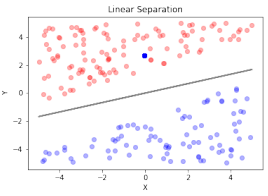
\includegraphics[scale=0.95]{linSep.png}\\
    \textbf{figure 1:} linear seperation\\
    
    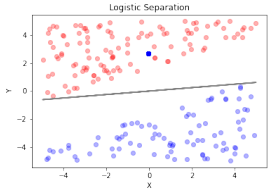
\includegraphics[scale=0.95]{logSep.png}\\
    \textbf{figure 2:} logistic seperation\\
  \end{center}

\end{enumerate}
 
\begin{Q}
  \textbf{\Large Robustness of the Majority Vote Classifier.}\\
  \def\maj{\textsc{Maj}}

   
   The purpose of this problem is to further investigate the behavior of the majority vote classifier using Hoeffding's inequality (\textit{this will be covered in the lecture 22, the Ensemble Methods lecture}).  Simplified versions of Hoeffding's inequality are as follows.
    \begin{theorem}\label{thm: hoeffding}
      Given independent random variables $(Z_1,\ldots,Z_k)$ with $Z_i \in [0,1]$,
        \begin{equation}\label{eq: hoeffding 1}
          \Pr\sbr{\sum_{i=1}^k Z_i \geq  \sum_{i=1}^k\mathbb{E}[Z_i] + k\eps } \leq \exp\del{-2k\eps^2},
        \end{equation}
        and
        \begin{equation}\label{eq: hoeffding 2}
          \Pr\sbr{\sum_{i=1}^k Z_i \leq  \sum_{i=1}^k\mathbb{E}[Z_i] - k\eps } \leq \exp\del{-2k\eps^2}.
        \end{equation}
    \end{theorem}

    In this problem we have an odd number $n$ of classifiers $\{f_1,\ldots,f_n\}$
    and only consider their behavior
    on a fixed data example $(\vx,y)$; by classifier we mean $f_i(\vx) \in \{\pm 1\}$.
    Define the majority vote classifer $\maj$ as
    \[
      \maj(\vx;f_1,\ldots,f_n)
      := 2\cdot \1\sbr{\sum_{i=1}^n f_i(\vx) \geq 0 } - 1
      = \begin{cases}
          +1 &\sum_{i=1}^n f_i(\vx) > 0, \\
          -1 &\sum_{i=1}^n f_i(\vx) < 0,
        \end{cases}
    \]
    where we will not need to worry about ties since $n$ is odd.

    To demonstrate the utility of \Cref{thm: hoeffding} in analyzing $\maj$, suppose
    that $\Pr[ f_i(\vx) = y ] = p > 1/2$ independently for each $i$.
    Then, by defining a random variable $Z_i := \1[ f_i(\vx) \neq y]$
    and noting $\bbE [Z_i] = 1 - p$,
    \begin{align*}
      \Pr[\maj(\vx;f_1,\ldots,f_n) \neq y]
      &=
      \Pr\sbr{ \sum_{i=1}^n \1[ f_i(\vx) \neq y] \geq \frac n 2 }
      \\
      &=
      \Pr\sbr{ \sum_{i=1}^n Z_i \geq n(1-p) - \frac n 2 + np }
      \\
      &=
      \Pr\sbr{ \sum_{i=1}^n Z_i \geq n \bbE [Z_1] + n(p-1/2) }
      \\
      &\leq
      \exp\del{ -2n(p-1/2)^2 }.
    \end{align*}
    The purpose of this problem is to study the behavior of $\maj(\vx)$ when not all of the classifiers $\{f_1,\ldots,f_n\}$ are independent.
    \begin{enumerate}
      \item
        Assume $n$ is divisible by $7$ and $5n/7$ is odd,
        and that of the $n$ classifiers $\{f_1,\ldots,f_n\}$,
        now only the first $5n/7$ of them (i.e., $\{f_1,\ldots,f_{5n/7}\}$) have independent errors on $\vx$.
        Specifically, $\Pr[f_i(\vx) = y] = p := 4/5$ for classifiers $\{f_1,\ldots,f_{5n/7}\}$.
        By contrast, we make no assumption on the other $2n/7$ classifiers (i.e., $\{f_{5n/7+1},\ldots,f_{n}\}$) and their errors. Now use Hoeffding's inequality to show that            
        \[
          \Pr\sbr{ \sum_{i=1}^{5n/7} \1[ f_i(\vx) \neq y] \geq \frac{3n}{14} }\le
         \exp\del{ -\frac{n}{70}  }.
   \]
   
     \item Continuing from (a), further show that the majority vote classifier
     over all $n$ classifiers is still good,  specifically showing  \[
     \Pr\sbr{ \maj(\vx;f_1,\ldots,f_n) \neq y } \leq \exp\del{ -\frac{n}{70}  }.
     \]
     
 
 \textbf{For full points:} You need to derive the inequality $\Pr\sbr{ \maj(\vx;f_1,\dots,f_n) \neq y } \leq \exp(-n / 70)$ rigorously for ANY possible behavior of the $\frac{2n}{7}$ arbitrary classifiers.


     \item Is the probability of correctly classifying $\vx$ reasonably good in part (b) for large $n$? Do you have any interesting observations? Any answer which contains at least one complete sentence will receive full credit.
    \end{enumerate}

\end{Q}
\begin{enumerate}
  \item let $Z_i:=\1 [f_i(x) \neq y]$, then we see that 
  $Pr[\sum_{i=1}^{5n/7} \1[f_i(x)\neq y] \geq \frac{3n}{14}] \\
  = Pr[\sum_{i=1}^{5n/7} Z_i \geq 5n/7(1-p) - 3n/14 + 5np/7]
  = Pr[\sum_{i=1}^{5n/5} Z_i \geq 5/7n \bbE[Z_1]+n(5p/7-3/14)]\\
  \leq \exp(-2*5/7n(5/7p-3/14)^2) = \exp(-\frac{n}{70})$

  \item $MAJ(x; f_1, . . . , f_n) = (\sum_{i=1}^{n} fi(x))$.
  Let $E_i$ denote the event that $f_i(x) \neq y$, and let $E_i^c$ denote the complement of $E_i$. Thus we have
  $Pr[M(x; f_1, . . . , f_n) \neq y] \leq Pr[\sum_{i=1}^{n} \1[E_i] > n/2] + Pr[\sum_{i=1}^{n} 1[E_i] = n/2]$
  By the union bound, we have
  $Pr[\sum_{i=1}^{n} \1[E_i] > n/2] \leq \sum_{i=1}^{n} Pr[E_i] = n(1-p)^{2n/7}$
  Similarly, we have
  $Pr[\sum_{i=1}^{n} 1[E_i] = n/2] \leq \sum_{i=1}^{n} Pr[E_i,E_i^c] \leq \sum_{i=1}^{n} Pr[E_i^c] = n/7$
  Combining the above inequalities, we have
  $Pr[M(x; f1, . . . , fn) \neq y] \leq n(1-p)^{2n/7} + n/7$
  Substituting $p = 4/5$ and simplifying the above expression, we get
  $Pr[M(x; f1, . . . , fn) \neq y] \leq \exp(-n/70)$
  
  \item The probability of correctly classifying $x$ using the majority vote classifier is very high for large 
  $n$ because the probability of making an error decreases exponentially with $n$ due to the negative exponential
\end{enumerate}
\end{enumerate}
\end{document}
